% filename: HEP_GL_OperationSafetyConcept

\documentclass{article}

\usepackage[utf8]{inputenc}
\usepackage[top=3cm, headheight=2.2cm, headsep=10pt]{geometry}
\usepackage{graphicx}

% To reference the last page
\usepackage{lastpage}

% Like `tabularx` but supports pagebreaks
\usepackage{ltablex}
% Adjust row vertical spacing
\renewcommand{\arraystretch}{1.2}

% Multiline cells
\usepackage{makecell}

% Set date format to ISO 8601
\usepackage{datetime}
\newdateformat{isodate}{\THEYEAR-\twodigit{\THEMONTH}-\twodigit{\THEDAY}}

% Table colouring
\usepackage[table,dvipsnames]{xcolor}
\definecolor{tableHeaderColor}
{rgb}{0.75,0.75,0.75}
\definecolor{tableColumnColor}
{rgb}{0.95, 0.95, 0.95}
\definecolor{notesColor}
{rgb}{0.95, 0.95, 0.95}
\definecolor{highlightColor}
{rgb}{1.00, 0.95, 0.80}

% Icons for checkbox
\usepackage{pifont}

% Command to create a checkbox
\newcommand{\checkbox}{\ding{113}}

% For automatic counters
\usepackage{array}

% Header and footer
\usepackage{fancyhdr}
\pagestyle{fancy}
\fancyhf{} % Clear header and footer
\renewcommand{\headrulewidth}{0pt}
\lhead{\includegraphics[width=2cm]{../../common/assets/HELIOS_LOGO.png}}
\rhead{\includegraphics[width=2cm]{../../common/assets/ARIS_space_to_grow_LOGO-black.pdf}}
\cfoot{\thepage}
\fancyfoot[L]{Project HEPHAESTUS}
\fancyfoot[C]{Page \thepage\ out of \pageref{LastPage}}

% Draft watermark
\newboolean{isDraft}
\setboolean{isDraft}{true} % Set to false to remove the watermark
\ifthenelse{\boolean{isDraft}}{
  \usepackage{background}
  \backgroundsetup{
    scale=25,
    color=gray,
    opacity=0.4,
    angle=45,
    position=current page.center,
    contents={Draft}
  }
}{}

% Highlight colour
\usepackage{soul}
\sethlcolor{magenta}

% Strikethrough
\usepackage[normalem]{ulem}

% Clickable Hyperlinks
\usepackage[colorlinks=true, linkcolor=blue, urlcolor=blue]{hyperref}

% Toggleable procedure items
\usepackage{etoolbox}



\title{Operation Safety Concept}
\author{Guideline}
\date{Version: \isodate\today}

\begin{document}

\maketitle

% Set the page style for the title page
\thispagestyle{fancy}

\section{Scope}

Within the framework of ETH Focus Project HEPHAESTUS, a Liquid Rocket Engine firing campaign is performed on the Dübendorf Airfield. The team members of project HEPHAESTUS received the permission from the Airfield to perform their tests. To ensure efficient and safe tests, this operational safety concept shall describe the test area and its available safety equipment and should give advice on how to behave during procedures and in emergencies.  
\\ \noindent
This document shall be read before each testing day by every visitor. 
With their signatures on the document HEP\_GL\_SafetySignature, all attendees confirm their knowledge of the general safety precautions and rules of behaviour according to this document. 

\section{Location of safety-relevant Institutions}
The contact information of the relevant safety institutions is listed in \ref{tab:safety-relevant-institutions}.
\begin{table}[h]
    \caption{Information of safety-relevant institutions}
    \label{tab:safety-relevant-institutions}
    \begin{tabularx}{0.9\textwidth}{|X|X|X|}
        \hline
        \rowcolor{tableHeaderColor} \textbf{Description} & \textbf{Address} & \textbf{Phone Number} \\ \hline
        Test Location & \begin{minipage}[t]{\linewidth}
            Flughafen Dübendorf – Hunter Stübli \\
            Rechweg \\
            8600 Dübendorf
            \vspace{1mm}
        \end{minipage} & - \\ \hline
        Spital Uster & \begin{minipage}[t]{\linewidth}
            Brunnenstrasse 42 \\
            8610 Uster
            \vspace{1mm}
        \end{minipage} & +41 44 911 11 11 \\ \hline
        Airfield Responsible & Roger Gisler & \begin{minipage}[t]{\linewidth}
            +41 58 481 79 18 \\
            If not reachable try: \\
            +41 79 944 42 52
            \vspace{1mm}
        \end{minipage} \\ \hline
        President ARIS & Chloé Pilloud & +41 79 226 39 42 \\ \hline
        Technical Advisor & Bruno Berger & +41 79 209 39 27 \\ \hline
    \end{tabularx}
\end{table}

In table \ref{tab:emergency-numbers} the emergency numbers are listed. Call them first before calling other relevant security institutions. In the case of an emergency, follow the contingency procedures as described in Section \ref{emergency-behaviour}.
\begin{table}[h]
    \caption{Emergency Numbers}
    \label{tab:emergency-numbers}
    \begin{tabularx}{0.9\textwidth}{|X|X|}
        \hline
        \rowcolor{tableHeaderColor} \textbf{Description} & \textbf{Phone Number} \\ \hline
        Ambulance & 144 \\ \hline
        Rega & 1414 \\ \hline
        Fire service & 118 \\ \hline
        Police & 117 \\ \hline
        Toxics & 145 \\ \hline
    \end{tabularx}
\end{table}
\section{Phases}
As scheduled in the Firing Conduction, every test is divided into the following phases:
\begin{enumerate}
    \item Pre-Preparation
    \item Preparation and Assembly
    \item Briefing
    \item Transfer to Airfield
    \textcolor{red}{
    \item Installation and Pre-Firing Checks
    \item Filling and Ignition Test
    \item Safe State Establishment}
    \item Post Firing Checks and Deinstallation
    \item Transfer to IPZ
    \item Disassembly and Inspection
    \item Debriefing
\end{enumerate}
The beginning of every phase needs to be clearly communicated to all attendees by the test conductor. Visitors shall keep a safe distance from the trailer during all phases. \\
\noindent
During phases 5 to 7, the system is in a dangerous state. Therefore, no one is allowed to leave the Hunter Stübli or designated area unless instructed to do so by the test conductor in order to execute a specific task.

\newpage

\section{Site Map}
The tests are performed in on the old runway of the Dübendorf Airfield. The area consists of the Runway, a hill and the Hunter Stübli (HUT). The trailer is positioned on the Runway in a way that the nozzle exhaust is pointed towards the hill. The Hunter Stübli is used as a control station. \\
\noindent
During test operations no external people should enter the entire area of the runway "Lili 15" from the mobile field hangar down to the Hunter-Stübli. If an attendee notices the approach of an unannounced person or of an animal, they are obliged to immediately inform the test conductor and/or the safety officer. If anyone enters the area an immediate abort is required. \\
\noindent
Figure \ref{fig:location-plan} shows the location of the emergency car, the meeting point (north of the emergency car), the pharmacy in the Hunterstübli and some fire extinguishers. The stop is to indicate that you should not drive through there. 
Figure \ref{fig:emergency-route} shows the route that should be driven to exit the airfield in case of an emergency, where the red route is the route through the official airport entrance and the blue arrow shows the exit through the gate.
\begin{figure}[h]
    \centering
    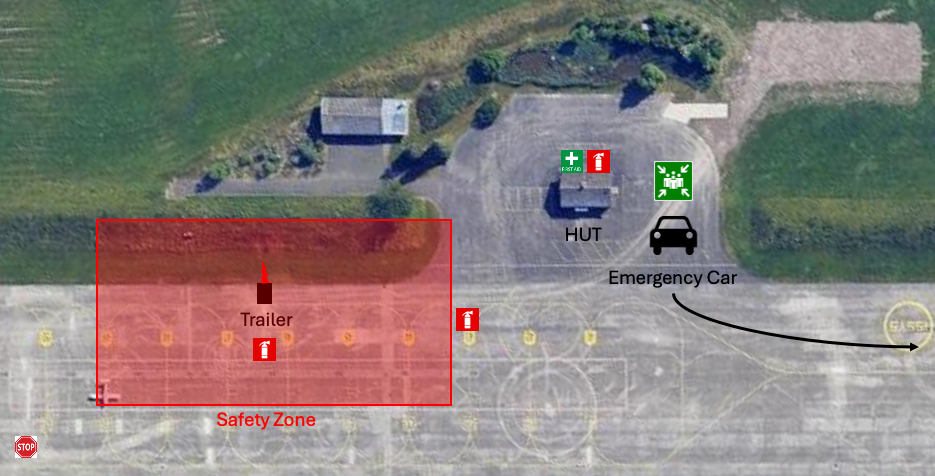
\includegraphics[width=\textwidth]{assets/location_map.png}
    \caption{Site map of the test location}
    \label{fig:location-plan}
\end{figure}

\newpage

\begin{figure}[h]
    \centering
    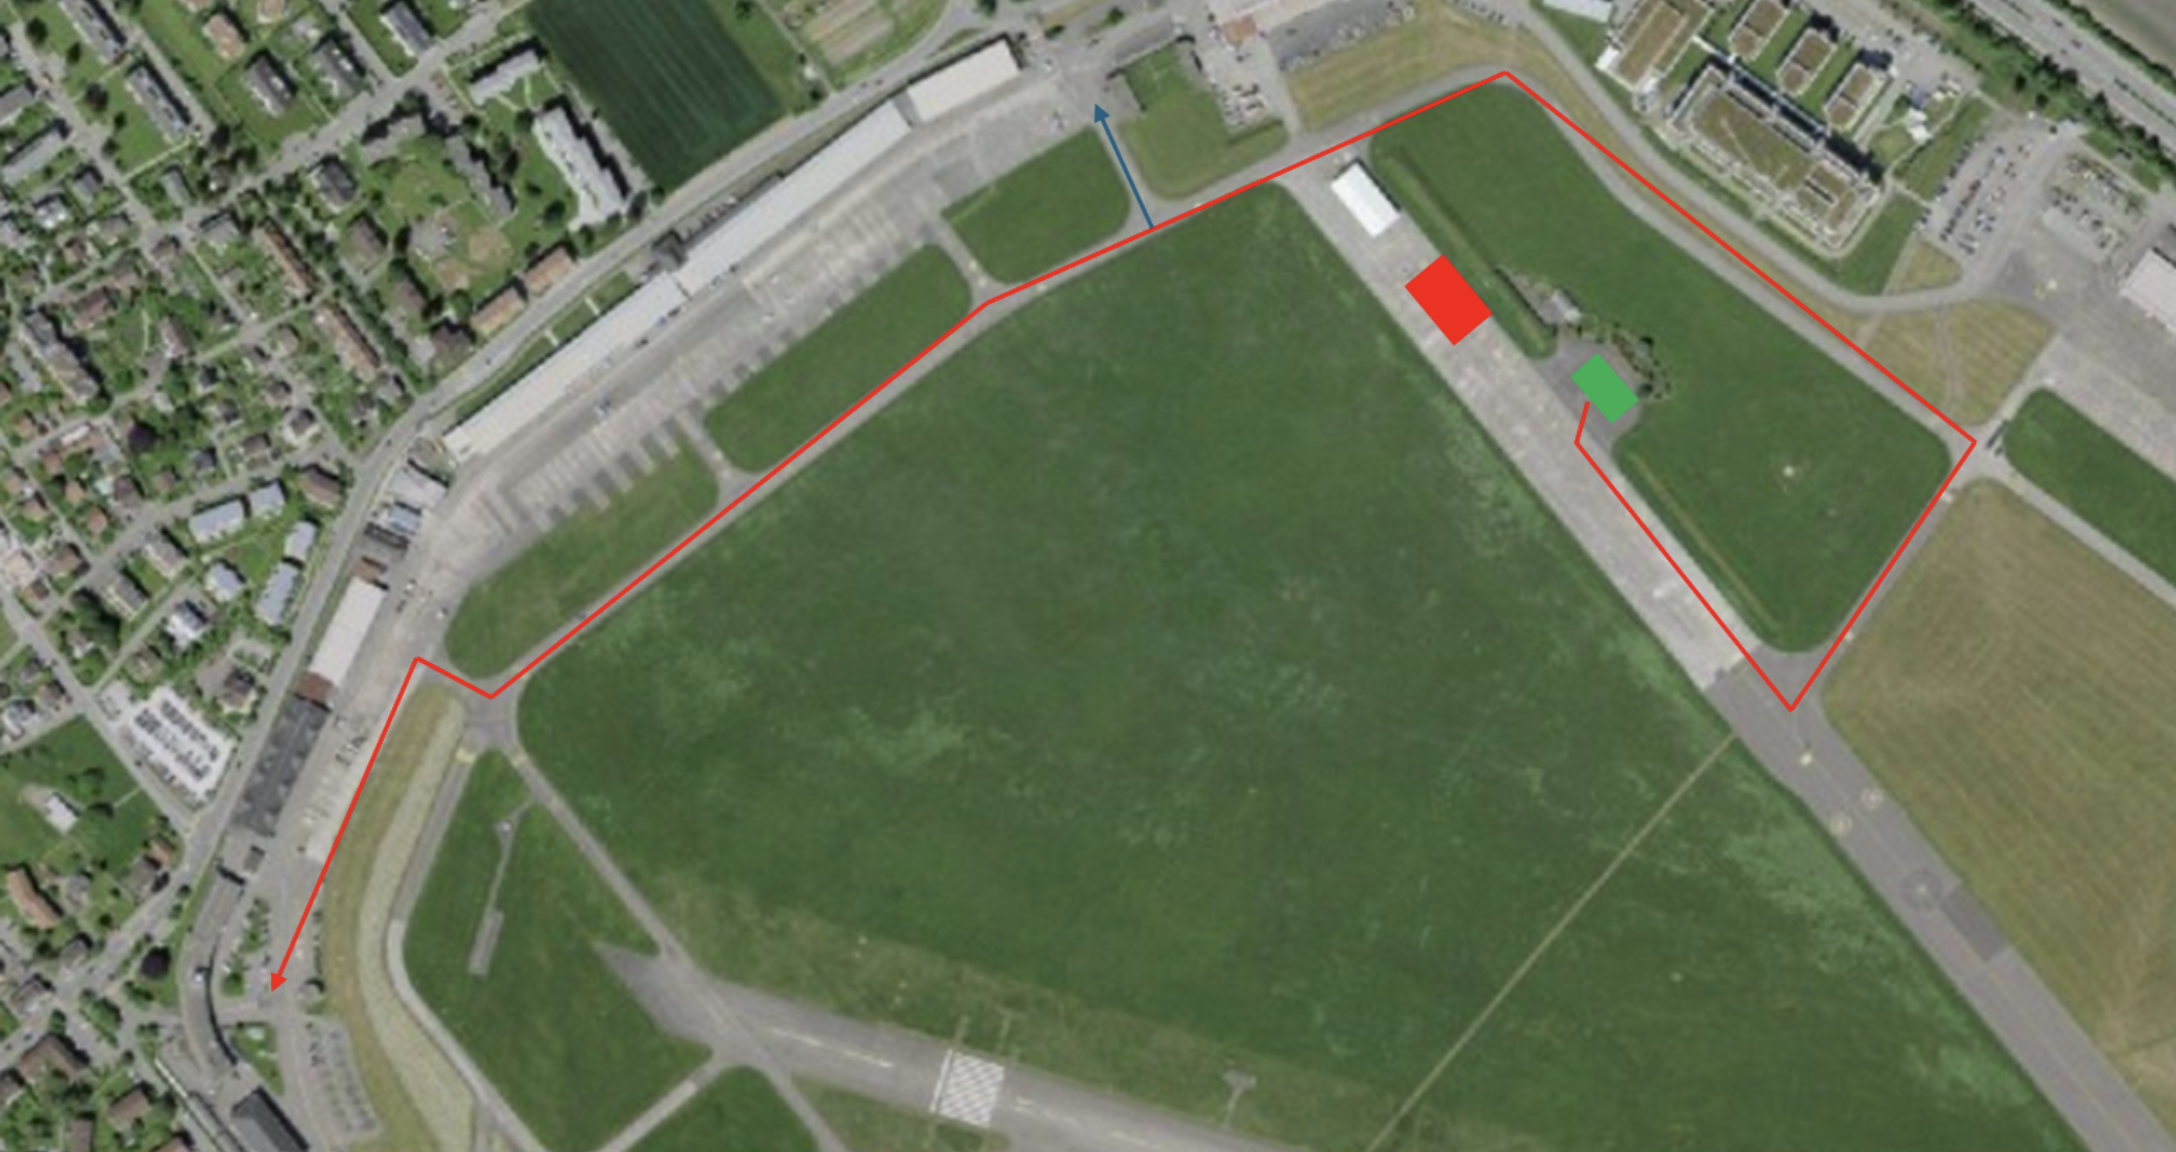
\includegraphics[width=\textwidth]{assets/emergency_route.png}
    \caption{Emergency route}
    \label{fig:emergency-route}
\end{figure}

\newpage
\section{Equipment}
Every person has to wear a warning vest according to their role at all times during testing operations. The color code displayed in table \ref{tab:color-code} is used.
\begin{table}[h]
    \caption{Warning Vest Color Code}
    \label{tab:color-code}
    \begin{tabularx}{0.9\textwidth}{|X|X|X|X|}
        \hline
        \cellcolor{cyan} Test Conductor & \cellcolor{green} Safety Officer & \cellcolor{orange} Engineers in charge (determined in role assignment) & \cellcolor{yellow} Visitors \\ \hline
    \end{tabularx}
\end{table}
The safety equipment is stored in the entrance of the HUT. The wearing of provided safety equipmentas foreseen in the operating procedures is mandatory.
\begin{table}[h]
    \caption{Safety Equipment}
    \label{tab:safety-equipment}
    \begin{tabularx}{0.9\textwidth}{|c|X|X|}
        \hline
        \rowcolor{tableHeaderColor} \textbf{Amount} & \textbf{Equipment} & \textbf{Comment} \\ \hline
        2 & Fire extinguisher & ABC-Pulver (in HUT and behind wall see Figure \ref{fig:location-plan}) \\ \hline
        2 & Fire extinguisher & CO2 (class B next to trailer) \\ \hline
        1 & First aid kit & Located in the HUT \\ \hline
        1 & Emergency car & Parked on the west side of the HUT and open, car key and gate key on driver's seat \\ \hline
        2 & Blue warning vest & \\ \hline
        2 & Green warning vest & \\ \hline
        10 & Yellow warning vest & \\ \hline
        6 & Orange warning vest & \\ \hline
        8 & Safety goggles & \\ \hline
        4 & Face shield & \\ \hline
        6 & Pair of safety shoes & \\ \hline
        2 & Pair of cold-resistant gloves & For handling gas and LOX \\ \hline
        1 & Blast shield & \\ \hline
        10 & Ear protection & \\ \hline
        2 & Cold-resistant faceshield & \\ \hline
        8 & Work gloves & \\ \hline
        2 & Barrier tape & \\ \hline
    \end{tabularx}
\end{table}

\section{Behaviour during test procedure}
The test conductor has the lead during the whole test operation and therefore gives the orders, which shall be obeyed. The safety officer supervises the actions of the test conductor and the team and makes sure that the tests are executed according to the procedures. The safety officer can stop the operations at any time he considers proceeding with the test as dangerous. \\
\noindent
If during the test procedure an anomaly occurs or if there is an insecurity, the test participants are requested to inform the test conductor and the safety officer immediately. \\
\noindent
The attendees are not allowed to take photos and record video material. A pre-determined photographer will take pictures and video footage. The publishing of this material via social media or other channels is strictly forbidden. All to be published material must be checked and approved by the Airfield Dübendorf on request of team HELIOS. \textbf{Please do not contact the Airfield on your own}. \\
\noindent
By signing the HEP\_GL\_SafetySignature you agree that during the tests pictures of you will be taken and used for internal purposes (photo gallery on website, flyer, Instagram, LinkedIn). If you do not agree, please contact the project manager or the safety officer during the briefing.
\begin{itemize}
    \item Focus
    \item Even if you know the steps by heart, follow the procedure so that nothing is forgotten 
    \item Work efficiently but do not rush. We’ll take all the time we need to do things properly
    \item If something does not go as planned or seems suspicious, inform the TC and SO. Better to delay the test than to damage the system or even injure someone
    \item If you notice unauthorized people, animals, cars, airplanes near the testing location, inform the TC and SO
    \item Wear safety equipment as specified in the procedures
    \item During every briefing all attendees must be present
    \item Between briefing and debriefing all present people outside of the HUT (on the airfield) are to wear safety goggles. Remind each other if someone forgets it
    \item Take care of each other
    \item In case of an incident: First, keep calm and think. Do not endanger yourself. Then react. Use the contingency procedures. Emergency responsibilities are defined
    \item Between briefing and debriefing all present people are to wear warning wests and Visitor Badges (military)
    \item Inform TC and SO when the task is completed
    \item There is a dedicated waiting area installed in the HUT, where you are encouraged to wait, if you have no current task
    \item Do not disturb/interrupt other working members
    \item No one is to leave the area visible from the HUT (as soon as we get there), except if explicitly demanded by an operation procedure or with the explicit consent of the TC or SO. Normal place to stay if there is no task is in the HUT
    \item When going to the toilet, let other people know
    \item You are NOT allowed to take any pictures or videos in HUT
    \item Please keep the tables, as well as all the working places empty and clean
\end{itemize}

\section{Behaviour in case of an emergency} \label{emergency-behaviour}
In case of an emergency or an unexpected system state, the contingency procedures (shown in table \ref{tab:contingency-procedures}) must be followed. Participants will be informed about the location of the contingency procedures during the briefing and installation according to the Firing Conduction.
\begin{table}[h]
    \caption{Contingency Procedures}
    \label{tab:contingency-procedures}
    \begin{tabularx}{0.9\textwidth}{|X|}
        \cellcolor{blue} \textcolor{white}{General} \\ \hline
        HEP\_CP\_GEN\_Injury\_XX \\ \hline
        HEP\_CP\_GEN\_Fire\_XX \\ \hline
        HEP\_CP\_GEN\_Trespassing\_XX \\ \hline
        \cellcolor{orange} PSS \\ \hline
        HEP\_CP\_PSS\_Leakage\_XX \\ \hline
        HEP\_CP\_PSS\_Overpressure\_XX \\ \hline
        HEP\_CP\_PSS\_BottleValve-Anomaly\_XX \\ \hline
        HEP\_CP\_PSS\_NoisesHissing\_XX \\ \hline
        \cellcolor{yellow} DACS \\ \hline
        HEP\_CP\_DACS\_PowerLoss\_XX \\ \hline
        HEP\_CP\_DACS\_ConnectionLoss\_XX \\ \hline
        HEP\_CP\_DACS\_ValveAnomalies\_XX \\ \hline
    \end{tabularx}
\end{table}
All attendees are guided to stay calm and to avoid panicking. In such a situation, communication needs to be reduced to the minimum / essential only. The safety officer or his substitute leads through all emergency situations supported by the test conductor. The roles of emergency drivers and emergency assistants are assigned already in advance and are clearly stated in the operating procedures and will be communicated during the briefing. The replacement in the event of a role failure is defined in the respective operating procedure and also clearly announced during the briefing. \\
\noindent
In any situation, the hazards must be considered before providing assistance. Particularly, the HUT must not be left without prior consideration of the state of the system! \\
\noindent
As soon as the situation allows it, the safety officer will inform Roger Gisler (Airfield Dübendorf), Chloé Pilloud (ARIS). Contacting a technical expert (Bruno Berger) can also be helpful in situations where expert advice or a technical assessment is needed. 
\end{document}